\documentclass[10pt,twocolumn]{article}

\usepackage[margin=0.78in]{geometry}
\usepackage{microtype}
\usepackage{amsmath,amssymb}
\usepackage{booktabs}
\usepackage{graphicx}
\usepackage{xcolor}
\usepackage{hyperref}
\usepackage{natbib}
\usepackage{enumitem}
\usepackage{array}

\hypersetup{
  colorlinks=true,
  linkcolor=blue!60!black,
  citecolor=blue!60!black,
  urlcolor=blue!60!black,
  pdftitle={Chatree: Organizing Long LLM Conversations as Branching Trees},
  pdfauthor={Shervin}
}

\setlength{\columnsep}{0.26in}
\setlist[itemize]{leftmargin=1.3em, itemsep=2pt, parsep=0pt, topsep=3pt}
\setlist[enumerate]{leftmargin=1.4em, itemsep=2pt, parsep=0pt, topsep=3pt}

\title{\textbf{Chatree: Organizing Long LLM Conversations as Branching Trees}}

\author{
  Shervin \\
  \texttt{https://github.com/shervinemp/Chatree}
}

\date{Technical Report --- v0.2.0}

\begin{document}
\maketitle

% ============================================================================
% ABSTRACT
% ============================================================================
\begin{abstract}
Long conversations with Large Language Models (LLMs) rarely move in a straight line. Users explore side questions, abandon dead ends, revise earlier decisions, and eventually run out of context space. Keeping everything in one flat transcript makes prompts grow on every turn and mixes rejected ideas with final choices. On the other hand, compressing history into rolling summaries or flat fact lists (such as Mem0) keeps prompts short, but permanently discards raw details the summarizer overlooked, loses track of which later decisions depend on an earlier spec, and breaks prompt prefix caching by rewriting the top of the prompt on every turn.

We present \textbf{Chatree}, a local-first framework that stores a conversation as a \textbf{tree of isolated branches} rather than a single linear log. Each side topic, exploratory spike, or continuation after compaction becomes its own branch. Branches keep their original messages intact in SQLite, generate a cheap summary plus a few dated facts when finished, and answer targeted cross-branch questions through isolated read-only lookups without polluting either chat. When a branch builds on another, Chatree records the dependency edge so a meaningful revision automatically flags downstream branches as out of date. Finally, all changing metadata (branch map, stale warnings, related pointers) is attached temporarily to the end of the latest user message, leaving earlier prompt bytes unchanged so provider KV caches continue to hit.

Across eight evaluation tracks on \texttt{deepseek-chat} against full-context chat, flat RAG, summary folding, official \texttt{mem0ai==2.2.1}, and official MIT \texttt{rlms==0.1.3}, Chatree ranks first on Official LoCoMo ($n=245$, \textbf{77.1\%} vs.\ 76.3\% linear and 73.5\% Mem0, at 5.5$\times$ smaller peak context) and Official LongMemEval-S ($n=30$, $\sim$115k-token histories, \textbf{80.0\%} vs.\ 70.0\% for linear, Mem0, and RLM, at 17.3$\times$ smaller peak context and 28\% lower total cost than Mem0). Across 9 successive compactions, Chatree retains \textbf{100\%} recall of un-anchored Turn-1 details while rolling summarization drops to \textbf{0\%}. Controlled zero-token traces and live head-to-head probes against Mem0 further verify 82.5\% vs.\ 0.7\% prefix cacheability, automatic multi-hop staleness flagging, and 0\% leakage from silently archived dead ends where unmodified Mem0 leaks abandoned prototype settings as active production configuration.
\end{abstract}

% ============================================================================
% 1. INTRODUCTION
% ============================================================================
\section{Introduction}

Anyone who uses an LLM for a multi-hour coding, debugging, or research session quickly hits the same wall: real work branches, but chat interfaces are flat. You spend twenty minutes debugging a gateway outage, pause to explore whether MongoDB might simplify your ledger, decide against it, return to your main design, revise an authentication timeout, and keep going until the context window fills up.

Current systems handle long conversations in one of two ways, and both break down:
\begin{enumerate}
  \item \textbf{Keep one growing linear chat.} Unrelated tangents and rejected ideas stay in the prompt forever. Every turn gets slower and more expensive, and models increasingly confuse old guesses with settled decisions as relevant details sink into the middle of long inputs \citep{liu2024lostinthemiddle}.
  \item \textbf{Distill history into summaries or flat facts.} Rolling compaction (e.g., in-place \texttt{/compact}) and memory layers like Mem0 \citep{chhikara2025mem0} shrink the active prompt, but at three steep costs: (a)~any exact detail the summarizer failed to extract at write time is gone for good; (b)~flat fact stores have no dependency graph, so revising an earlier decision never warns you that downstream configs are now broken; and (c)~injecting freshly retrieved memories near the start of the prompt mutates byte~0 on every turn, defeating provider KV-cache reuse \citep{zheng2024sglang}.
\end{enumerate}

\paragraph{A Concrete Example.}
Consider a small four-branch engineering session:
\begin{itemize}
  \item \textbf{Branch A (Auth):} Settles \texttt{JWT\_TTL=60m} and \texttt{RS256}.
  \item \textbf{Branch B (Edge Cache):} Imports Branch~A and sets \texttt{CACHE\_TTL=30m} (must stay $\le$ half of \texttt{JWT\_TTL}).
  \item \textbf{Branch C (Mobile Refresh):} Imports Branch~B and sets \texttt{REFRESH\_WINDOW=25m} (5 minutes below \texttt{CACHE\_TTL}).
  \item \textbf{Branch D (MongoDB Spike):} Explores \texttt{MongoDB 7.0} with replica set \texttt{rs\_ledger\_0} for four turns, then gets closed and archived without writing a formal cancellation essay.
\end{itemize}
Later, a security review revises \emph{only} Branch~A to \texttt{JWT\_TTL=10m} and \texttt{ED25519}. In a flat chat, all four threads sit interleaved in one growing transcript. In a flat fact store, Branch~D's MongoDB parameters remain active memories because nobody typed ``cancel MongoDB,'' and neither Branch~B nor Branch~C receives any signal that its cached assumptions just became unsafe.

\paragraph{Our Approach.}
Chatree treats a conversation like a tree of lightweight branches—closer to Git branches than a scrolling chat log—built around four straightforward ideas:
\begin{enumerate}
  \item \textbf{Isolate branches and never destroy history.} Side topics run in child branches that inherit either the full parent history, the last few turns, or a clean slate. Abandoned branches are marked \texttt{ARCHIVED}, immediately hiding them from active search without deleting the audit trail. When a branch grows too long, Chatree hands a compact checkpoint to a fresh child branch and leaves the old branch intact.
  \item \textbf{Keep cheap summaries for search, but ask the original branch for exact details.} Finishing a branch generates a short summary and extracts up to 8 dated facts in the same LLM call (zero extra calls). When a later question needs an exact port, error code, or config line that never made it into the summary, Chatree sends a \emph{read-only question} directly to that branch over its verbatim turns and caches the answer.
  \item \textbf{Track causal dependencies across branches.} Whenever Branch~B reads from or imports Branch~A, Chatree records a directed edge $A \to B$. If Branch~A is later revised in a substantive way (changing identifiers, numbers, or polarity rather than minor wording), Chatree walks the dependency graph and flags both B (1~hop) and C (2~hops) as stale.
  \item \textbf{Append changing metadata at the tail, never the prefix.} Every branch's past messages stay byte-for-byte frozen. Dynamic orientation (neighboring branches, stale alerts, recent jumps, related hints) is attached temporarily to the newest user turn and discarded before the next turn, keeping the static prefix intact for KV caching.
\end{enumerate}

We implement Chatree as an open-source, provider-agnostic Python library over a single local SQLite database and evaluate it across eight tracks—including Official LoCoMo ($n=245$), Official LongMemEval-S ($n=30$), non-monotonic engineering workspaces, 9-generation compaction, live natural-prompt chats, and targeted simulations and live probes against unmodified \texttt{mem0ai==2.2.1} and MIT \texttt{rlms==0.1.3}. We also document clearly where a tree is \emph{not} worth the overhead: on short linear threads under $\sim$10k tokens, plain chat is simpler and cheaper.

% ============================================================================
% 2. HOW CHATREE WORKS
% ============================================================================
\section{How Chatree Works}

Figure~\ref{fig:arch} gives an overview of the system. Everything lives in one local SQLite database (with FTS5 full-text search and local embeddings), requiring no external database server.

\begin{figure*}[t]
  \centering
  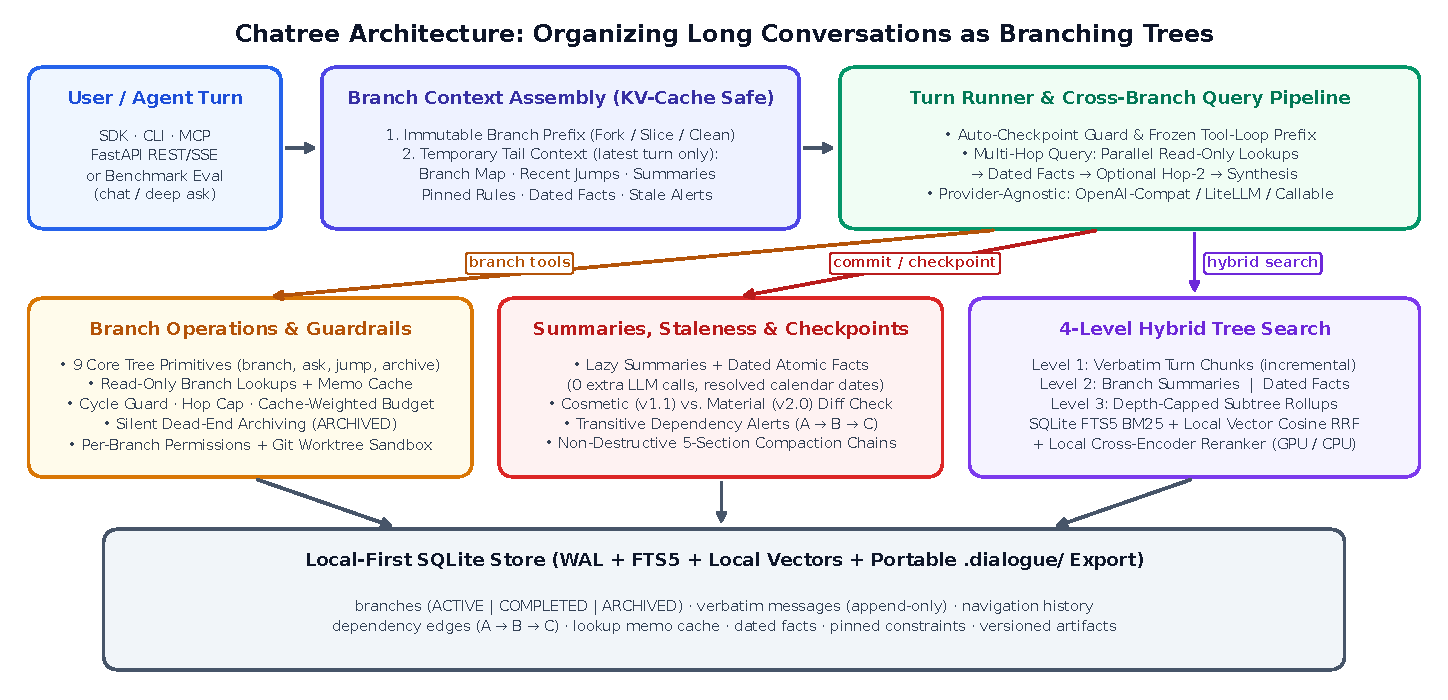
\includegraphics[width=\textwidth]{figures/fig1_architecture.pdf}
  \caption{Overview of Chatree. Each branch maintains an immutable prefix for KV caching and receives dynamic tree context only at the tail of the active turn. Cross-branch reads use cached summaries or read-only lookups over verbatim history, while SQLite stores messages, summaries, dated facts, dependency edges, and archived branches.}
  \label{fig:arch}
\end{figure*}

\subsection{Branches, Archiving, and Non-Destructive Checkpoints}
Each node in a Chatree workspace represents one focused thread and stores: (i)~its parent link and status (\texttt{ACTIVE}, \texttt{COMPLETED}, or \texttt{ARCHIVED}); (ii)~its append-only verbatim message list; (iii)~a lazily updated summary with a version number and up to 8 dated facts; (iv)~optional versioned text artifacts (such as specs or code snippets); and (v)~directed dependency edges to branches it has read from. Users and agents move between branches using a Git-style navigation history (\texttt{back}, \texttt{forward}, or \texttt{HEAD@\{k\}}), and multiple independent cursors can inspect the same tree concurrently.

When spawning a child branch $c$ from parent $u$ at message index $k$, the caller chooses one of three context modes:
{\small
\begin{equation}
  P(c) = \begin{cases}
    P(u)\Vert M_{1..k}(u) \Vert M(c), & \text{fork},\\
    S_{\text{sys}} \Vert b(c) \Vert M_{k-w+1..k}(u) \Vert M(c), & \text{slice},\\
    S_{\text{sys}} \Vert b(c) \Vert M(c), & \text{clean},
  \end{cases}
\end{equation}}
\noindent where $S_{\text{sys}}$ is the system prompt, $b(c)$ is a short brief frozen at branch creation, $M(\cdot)$ denotes verbatim messages, and \texttt{slice} inherits the last $w$ parent turns. Fork points automatically align to completed tool-call boundaries so no branch ever inherits an orphaned tool request.

\paragraph{Dead-End Archiving.}
Closing a dead-end exploration sets its status to \texttt{ARCHIVED}. Archived branches are excluded immediately from every search index and summary overview—without asking the user to type a cancellation note—while remaining preserved in SQLite if anyone explicitly inspects the audit log.

\paragraph{Non-Destructive Compaction.}
When a branch exceeds its token limit, Chatree does not overwrite or delete older turns. Instead, it writes a concise 5-section handoff (objective, locked decisions and exact identifiers, verified artifacts, rejected options, and next steps) using the branch's warm prefix, marks the original branch \texttt{COMPLETED}, and continues work in a fresh child branch linked back to its predecessor ($B_1 \to B_2 \to \dots \to B_k$). If keeping recent turns would fail to shrink context, Chatree automatically steps down from \texttt{slice} to \texttt{clean} mode. Because every ancestor remains untouched, an agent in $B_9$ can still recover an un-anchored detail from Turn~1 of $B_1$.

\subsection{Two-Level Retrieval: Cheap Index Plus Read-Only Branch Lookups}
To keep common queries fast while guaranteeing lossless fallback, Chatree indexes active branches at four granularities using hybrid BM25 + dense vector retrieval (fused via Reciprocal Rank Fusion \citep{cormack2009rrf} and optionally reranked with a small local cross-encoder):
\begin{itemize}
  \item \textbf{Verbatim chunks:} Sliding windows of raw turns prefixed with the branch title and goal \citep{anthropic2024contextual}, indexed incrementally as messages arrive.
  \item \textbf{Branch summaries:} Generated lazily when a branch finishes or is queried. For long cold branches, a role-balanced trimmer caps input at 7,500 characters while keeping all user turns intact and splitting remaining space evenly across assistant replies so late turns are never dropped.
  \item \textbf{Dated atomic facts (zero extra LLM calls):} The same summary prompt asks the model to emit a small JSON list of up to 8 speaker-attributed facts with relative dates (``yesterday,'' ``two weeks ago'') resolved to explicit calendar dates using the session's weekday-anchored timestamp. Because facts stay scoped to their branch, they never destructively overwrite facts in other branches.
  \item \textbf{Subtree rollups:} Lightweight upward summaries (depth-capped at 8) for coarse discovery in large trees.
\end{itemize}

\paragraph{Read-Only Branch Lookups (Shadow Turns).}
When a branch needs information from another branch $v$:
\begin{enumerate}
  \item If no specific question is asked and $v$'s summary is up to date, Chatree returns the cached summary for \textbf{0 LLM tokens}.
  \item If a specific question $q$ is asked, Chatree first checks a memoization cache keyed by $(v, \text{message count}, \text{model})$ using both exact normalized hashes and cosine similarity ($\ge 0.90$) guarded by exact identifier matching (so a cached answer for \texttt{PORT\_8080} is never returned for \texttt{PORT\_8081}).
  \item On a cache miss, Chatree runs an isolated \textbf{read-only query} over $v$'s verbatim history—blocking any state-changing tools and wrapping the reply as untrusted data—then caches the answer and logs a dependency edge from the caller to $v$. If $v$ is the tip of a compacted chain ($B_k$) and does not contain the detail locally, Chatree automatically walks back up the chain ($B_{k-1} \dots B_1$) in one bounded hop and caches the resolved answer under $B_k$.
\end{enumerate}

For complex cross-branch questions (both in live calls and external benchmarks), a single shared query pipeline runs in four steps: (1)~retrieve top candidate branches and run parallel read-only lookups; (2)~pull matching dated facts at 0 LLM cost; (3)~optionally run a second drill-down pass over remaining branches when the first pass is incomplete or the question involves multi-session counting, comparison, or updates; and (4)~synthesize a chronologically ordered answer.

\subsection{Dependency Tracking and Staleness Alerts}
Dependency edges are recorded automatically whenever a branch queries another branch or imports up to 4 sibling snapshots at spawn time (frozen into the new branch's brief). When an upstream branch $v$ is later reopened and edited, Chatree checks whether the new summary changed concrete identifiers, numbers, or polarity (e.g., ``enabled'' $\to$ ``disabled''):
\begin{itemize}
  \item \textbf{Cosmetic edits} bump a minor version ($v1.1$) and trigger no alerts, avoiding alert fatigue.
  \item \textbf{Material revisions} bump a major version ($v2.0$), record a one-line diff (e.g., \texttt{removed [60m, RS256]; added [10m, ED25519]}), and run a cycle-safe breadth-first walk across recorded dependencies to mark both direct consumers ($B$, 1~hop) and transitive consumers ($C$, 2~hops) stale.
\end{itemize}
Tree-wide pinned invariants (up to 8 shared constraints, such as an active latency SLO) also track their source branch and are flagged \texttt{[STALE]} if that branch is revised or archived.

\subsection{Preserving Prompt KV Caches}
Hosted LLM providers and serving engines like SGLang \citep{zheng2024sglang} cache attention keys and values strictly from byte~0 onward: changing a single token near the start of the prompt forces recomputing the entire conversation. Chatree protects this prefix with three simple rules:
\begin{enumerate}
  \item \textbf{Freeze historical messages and titles:} A branch's opening brief binds to a frozen initial label, so automatic background titling updates the UI and search headers without touching prompt bytes.
  \item \textbf{Inject dynamic context at the tail only:} Topology, recent branch jumps, stale alerts, pinned invariants, and search hints are placed inside a temporary XML block on the \emph{latest} user message and stripped before saving to SQLite.
  \item \textbf{Keep tool definitions identical:} Read-only lookups send the same tool-schema array as active turns (blocking mutating tools in code rather than changing the schema prefix), avoiding byte-0 cache misses.
\end{enumerate}

\subsection{Implementation Notes}
Chatree is implemented in Python~3.12 over SQLite (WAL mode + FTS5) with a zero-dependency OpenAI-compatible HTTP/SSE client alongside optional LiteLLM routing, a CLI, a stdio MCP server, and an optional FastAPI + React explorer. Cross-branch calls are guarded by cycle detection, a hop-depth cap, and a token budget ledger that weights cached input tokens at 0.1$\times$. Local retrieval uses \texttt{BAAI/bge-small-en-v1.5} embeddings and an optional \texttt{ms-marco-MiniLM-L-6-v2} cross-encoder with automatic GPU-to-CPU fallback. The core codebase is covered by 111 automated tests requiring no API keys.

% ============================================================================
% 3. RELATED WORK
% ============================================================================
\section{Related Work}

\paragraph{Long Context and Flat RAG.}
Modern models advertise 128k--1M context windows \citep{deepseek2024v3}, but accuracy still degrades when key facts sit in the middle of long histories \citep{liu2024lostinthemiddle} and prefill cost grows with every turn. Flat chunk RAG \citep{lewis2020rag,anthropic2024contextual} bounds prompt size, yet breaks multi-turn threads into isolated fragments with no notion of branching, superseded specs, or archived dead ends.

\paragraph{Agent Memory Systems.}
MemGPT/Letta \citep{packer2023memgpt} pages turns out of a small working window into archival search, but summarizes and evicts turns destructively. Mem0 \citep{chhikara2025mem0} runs dedicated LLM calls on every write to extract and reconcile discrete facts in a vector/graph store; this produces very small query prompts, but throws away verbatim transcripts, offers no dependency tracking or branch archiving, and disrupts prefix caching. Zep/Graphiti \citep{rasmussen2025zep} builds a bi-temporal knowledge graph for fact validity intervals, whereas Chatree keeps raw conversations as queryable branches and piggybacks lightweight dated facts onto branch summaries at zero extra LLM calls.

\paragraph{Tree Inference and Prefix Caching.}
Tree-of-Thoughts \citep{yao2023tot} branches within a single reasoning problem rather than managing persistent multi-turn dialogue. Recursive Language Models (RLM) \citep{zhang2025rlm} expose transcripts to a Python REPL for lossless programmatic inspection, but incur multi-iteration latency and 0\% KV-cache reuse. SGLang RadixAttention \citep{zheng2024sglang} shares KV prefixes across branches inside the inference engine; Chatree complements serving-layer caching by keeping prompts prefix-stable at the application layer. Table~\ref{tab:capabilities} summarizes these trade-offs.

\begin{table*}[t]
\centering
\caption{Feature comparison across long-horizon conversational memory approaches.}
\label{tab:capabilities}
\small
\setlength{\tabcolsep}{3.5pt}
\resizebox{\textwidth}{!}{%
\begin{tabular}{@{}lccccccccc@{}}
\toprule
\textbf{Capability} & \textbf{Linear} & \textbf{Sliding} & \textbf{Flat RAG} & \textbf{Mem0} & \textbf{Letta} & \textbf{Zep/Graphiti} & \textbf{Folding} & \textbf{MIT RLM} & \textbf{Chatree} \\
\midrule
Bounded $O(1)$ working context     & $\times$ & \checkmark & \checkmark & \checkmark & \checkmark & \checkmark & \checkmark & Partial & \textbf{\checkmark} \\
Lossless verbatim ancestor recall  & \checkmark$^\dagger$ & $\times$ & Partial & $\times$ & Partial & Partial & $\times$ & \checkmark & \textbf{\checkmark (Lookup)} \\
Branching \& dead-end archiving    & $\times$ & $\times$ & $\times$ & $\times$ & $\times$ & $\times$ & Partial & $\times$ & \textbf{\checkmark} \\
Transitive staleness tracking      & $\times$ & $\times$ & $\times$ & $\times$ & $\times$ & Temporal & $\times$ & $\times$ & \textbf{\checkmark} \\
Non-destructive compaction         & $\times$ & $\times$ & $\times$ & $\times$ & Destr. & $\times$ & Destr. & N/A & \textbf{\checkmark} \\
Dated atomic facts                 & $\times$ & $\times$ & $\times$ & Extra LLM & $\times$ & KG & $\times$ & $\times$ & \textbf{\checkmark (0 extra calls)} \\
KV-cache prefix preservation       & \checkmark & $\times$ & $\times$ & $\times$ & Partial & $\times$ & Partial & $\times$ & \textbf{\checkmark (31--83\%)} \\
Git-style branch navigation        & $\times$ & $\times$ & $\times$ & $\times$ & $\times$ & $\times$ & $\times$ & $\times$ & \textbf{\checkmark} \\
\bottomrule
\multicolumn{10}{@{}l}{\footnotesize $^\dagger$Linear chat retains verbatim history only until the model's context window overflows.}
\end{tabular}%
}
\end{table*}

% ============================================================================
% 4. EXPERIMENTAL SETUP
% ============================================================================
\section{Experimental Setup}

\paragraph{Models and Local Retrieval.}
All live runs use \texttt{deepseek-chat} \citep{deepseek2024v3} paired with local embeddings (\texttt{bge-small-en-v1.5}, 384-dim) and cross-encoder reranking (\texttt{ms-marco-MiniLM-L-6-v2}) on a single RTX~4080 Laptop GPU (zero embedding API cost). No gold session summaries are provided to any system.

\paragraph{Baselines.}
We test unmodified upstream releases alongside standard baselines:
\begin{itemize}
  \item \textbf{Full Linear:} Entire history up to 120k tokens with prompt caching enabled.
  \item \textbf{Mem0 (Official):} Unmodified \texttt{mem0ai==2.2.1} using the same \texttt{deepseek-chat} model and local \texttt{bge-small-en-v1.5} embeddings (\texttt{top\_k=8}).
  \item \textbf{MIT RLM (Official):} Unmodified \texttt{rlms==0.1.3} \citep{zhang2025rlm} (\texttt{max\_depth=1}, up to 8 iterations).
  \item \textbf{Flat Hybrid RAG:} Chunk-level BM25 + dense vector RRF + cross-encoder reranking (\texttt{top\_k=5}).
  \item \textbf{Summary Folding:} Branch summaries only, without read-only lookups over raw turns.
  \item \textbf{Sliding Window \& Destructive Rolling:} Recency-window and in-place compaction baselines.
\end{itemize}

\paragraph{Benchmarks and Metrics.}
We evaluate eight tracks grouped around four questions:
\begin{enumerate}
  \item \textbf{Long-horizon memory benchmarks:} Official \textbf{LoCoMo} (ACL 2024 \citep{maharana2024locomo}; stratified macro-balanced 5 QAs/category across all 10 conversations, 272 sessions, $n=245$ QAs) and Official \textbf{LongMemEval-S} (ICLR 2025 \citep{wu2025longmemeval}; 5 items per official category, $n=30$, 1,429 sessions, $\sim$115k tokens per item).
  \item \textbf{Targeted diagnostics vs.\ Mem0 (Track~8):} A zero-API-token structural trace running real Chatree and real \texttt{mem0ai==2.2.1} through a local proxy (16-turn prefix cache stability, write-prompt scaling, and 3 identical-lossiness probes), followed by a live \texttt{deepseek-chat} run of the exact same 3 probes ($\sim$\$0.015).
  \item \textbf{Compaction and live multi-turn chats (Tracks~5 \&~6):} A 9-generation compaction benchmark testing both anchored decisions and un-anchored Turn-1 diagnostics, plus an 18-turn live jump-around chat using plain natural prompts with zero tool jargon.
  \item \textbf{Controlled stress suites, ablations, and scaling (Tracks~1, 2, \&~7):} Five stress scenarios, 10 single-feature ablations, a $K \in \{2,4,8\}$ distractor sweep, and a 6-project non-monotonic software engineering benchmark ($n=36$, 80 sessions).
\end{enumerate}
For external benchmarks, we report both query cost and write-time ingest cost (\textbf{Total Lifecycle USD}), 95\% bootstrap confidence intervals (10,000 resamples), and exact two-sided paired McNemar $p$-values \citep{mcnemar1947note}.

% ============================================================================
% 5. RESULTS
% ============================================================================
\section{Results}

\subsection{Long-Horizon Memory Benchmarks: LoCoMo and LongMemEval-S}

\paragraph{Official LoCoMo ($n=245$).}
Table~\ref{tab:locomo} and Figure~\ref{fig:locomo} report 7-system results on LoCoMo under a fixed adversarial rubric that separates distractor answers from ground truth and credits truthful false-premise corrections.

\begin{table*}[t]
\centering
\caption{Official LoCoMo ($n=245$ stratified QAs across 10 conversations / 272 sessions; \texttt{deepseek-chat}). Total USD breaks down query + write-time ingest cost (\texttt{Q+I}). Bold marks best per column; $^*$ denotes $p < 0.05$ by exact paired McNemar test vs.\ Chatree. $\ddagger$Partial checkpoint ($n=117$); McNemar computed over the exact 117-QA intersection.}
\label{tab:locomo}
\small
\setlength{\tabcolsep}{3.0pt}
\resizebox{\textwidth}{!}{%
\begin{tabular}{@{}lrcccccccrrrc@{}}
\toprule
\textbf{System} & \textbf{$n$} & \textbf{Overall (95\% CI)} & \textbf{Sgl} & \textbf{Mlt} & \textbf{Tmp} & \textbf{Opn} & \textbf{Adv} & \textbf{Peak} & \textbf{Total USD (Q+I)} & \textbf{p95} & \textbf{Cache} & \textbf{$p$} \\
\midrule
\textbf{Chatree (Full)} & 245 & \textbf{77.1\%} {\scriptsize[71.8, 82.5]} & 86\% & 80\% & 74\% & \textbf{58\%} & 86\% & 6,390 & \$1.04 {\scriptsize(.84+.20)} & 7.8s & 60.0\% & ref \\
Full Linear & 245 & 76.3\% {\scriptsize[71.4, 82.0]} & \textbf{88\%} & \textbf{82\%} & 68\% & 56\% & 86\% & 35,097 & \$0.30 {\scriptsize(.30+.00)} & 3.1s & \textbf{95.4\%} & .874 \\
Mem0 (\texttt{2.2.1}) & 245 & 73.5\% {\scriptsize[68.2, 79.2]} & 78\% & 66\% & 74\% & 53\% & 94\% & 874 & \$0.20 {\scriptsize(.05+.15)} & \textbf{2.4s} & 0.1\% & .223 \\
MIT RLM (\texttt{0.1.3})$^\ddagger$ & 117 & 70.9\% {\scriptsize[62.4, 78.6]} & 76\% & 64\% & \textbf{80\%} & 55\% & 77\% & 28,166 & \$1.38 {\scriptsize(1.38+.00)} & 28.3s & 0.0\% & .473 \\
Chatree (no dated facts) & 245 & 64.5\% {\scriptsize[58.8, 70.6]} & 78\% & 50\% & 52\% & 44\% & \textbf{96\%} & 4,250 & \$0.67 {\scriptsize(.57+.10)} & 8.4s & 75.5\% & \textbf{.0001$^*$} \\
Flat Hybrid RAG & 245 & 48.2\% {\scriptsize[42.0, 54.3]} & 46\% & 26\% & 40\% & 33\% & 94\% & \textbf{725} & \textbf{\$0.05} {\scriptsize(.05+.00)} & 3.1s & 2.3\% & \textbf{$<$.0001$^*$} \\
Summary Folding & 245 & 41.2\% {\scriptsize[35.5, 47.3]} & 40\% & 32\% & 16\% & 31\% & 86\% & 1,480 & \$0.06 {\scriptsize(.06+.00)} & \textbf{2.1s} & 11.9\% & \textbf{$<$.0001$^*$} \\
\bottomrule
\end{tabular}%
}
\end{table*}

\begin{figure*}[t]
  \centering
  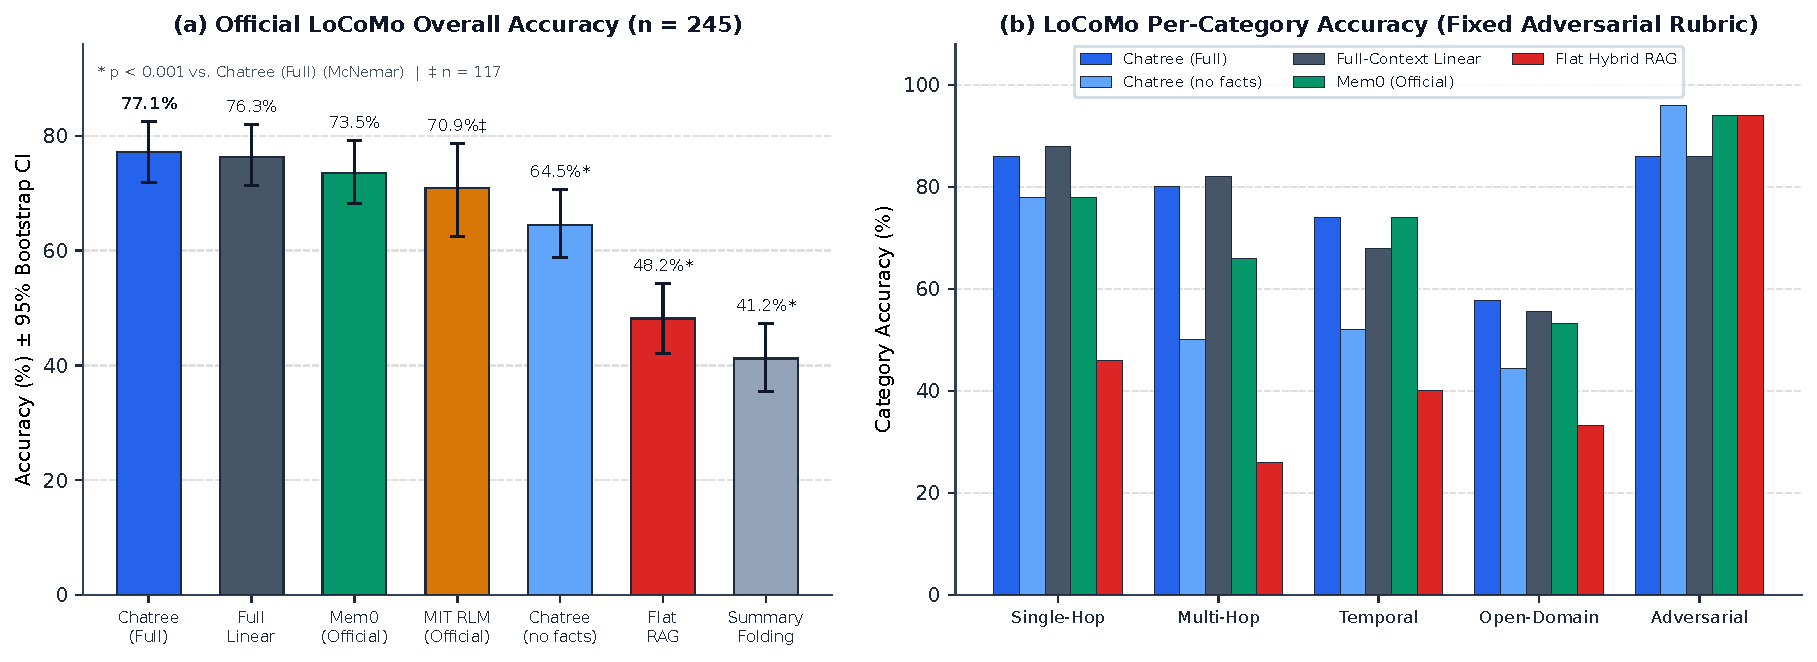
\includegraphics[width=\textwidth]{figures/fig2_locomo_comparison.pdf}
  \caption{Official LoCoMo ($n=245$): (a)~overall accuracy with 95\% bootstrap CIs and paired McNemar tests vs.\ Chatree; (b)~per-category accuracy showing the +30~pt multi-hop and +22~pt temporal jump from piggybacked dated facts.}
  \label{fig:locomo}
\end{figure*}

Three takeaways stand out on LoCoMo:
\begin{itemize}
  \item \textbf{Highest overall accuracy at 5.5$\times$ smaller peak context:} Chatree scores \textbf{77.1\%}, edging out Full Linear (76.3\%) while capping peak context at 6,390 vs.\ 35,097 tokens, and beating Flat RAG (+28.9~pts, $p<10^{-4}$) and Summary Folding (+35.9~pts, $p<10^{-4}$).
  \item \textbf{Clear multi-hop edge over Mem0 and RLM:} Chatree outperforms Mem0 (73.5\%) by \textbf{+14.0~pts on multi-hop} (80\% vs.\ 66\%) and \textbf{+8.0~pts on single-hop} (86\% vs.\ 78\%) while keeping \textbf{60.0\% KV-cache hits} vs.\ Mem0's 0.1\%. Mem0 remains faster per query (p95 2.4s vs.\ 7.8s) and cheaper at this 35k-token scale, though 75\% of Mem0's bill already goes to write-time extraction (\$0.153 ingest vs.\ \$0.051 queries).
  \item \textbf{Piggybacked dated facts matter ($p=0.0001^*$):} Extracting dated facts inside the existing summary pass lifts accuracy by \textbf{+12.6~pts} (64.5\% $\to$ 77.1\%) with zero extra write-time LLM calls, led by +30~pts on multi-hop and +22~pts on temporal questions.
\end{itemize}

\paragraph{Official LongMemEval-S ($n=30$, $\sim$115k Tokens/Item).}
As conversations grow past 100k tokens (Table~\ref{tab:lme} and Figure~\ref{fig:pareto}), the trade-offs shift sharply in Chatree's favor.

\begin{table*}[t]
\centering
\caption{Official LongMemEval-S ($n=30$, 5 items per category, $\sim$48 sessions / $\sim$115k tokens per item, 1,429 sessions total). Reporting Total Lifecycle USD (\texttt{Q+I}) exposes write-time extraction cost: Mem0 spends \$1.546 on ingest vs.\ \$0.009 on queries (176$\times$), making it 28\% more expensive overall than Chatree while trailing by 10~pts overall and 40~pts on \texttt{knowledge-update}.}
\label{tab:lme}
\small
\setlength{\tabcolsep}{3.0pt}
\resizebox{\textwidth}{!}{%
\begin{tabular}{@{}lcccccccrrcr@{}}
\toprule
\textbf{System} & \textbf{Overall (95\% CI)} & \textbf{S-User} & \textbf{S-Asst} & \textbf{Pref} & \textbf{Update} & \textbf{Temp.} & \textbf{Multi} & \textbf{Peak Tok} & \textbf{Total USD (Q+I)} & \textbf{p50 / p95} & \textbf{$p$ vs.\ Ref} \\
\midrule
\textbf{Chatree (Full)} & \textbf{80.0\%} {\scriptsize[66.7, 93.3]} & 80\% & \textbf{100\%} & \textbf{100\%} & 80\% & 60\% & \textbf{60\%} & 6,295 & \$1.12 {\scriptsize(.23+.88)} & 5.1 / 7.7s & ref \\
Full Linear & 70.0\% {\scriptsize[53.3, 86.7]} & \textbf{100\%} & \textbf{100\%} & 20\% & \textbf{100\%} & 60\% & 40\% & 108,772 & \$0.88 {\scriptsize(.88+.00)} & 2.4 / 4.8s & 0.5078 \\
Mem0 (\texttt{2.2.1}) & 70.0\% {\scriptsize[53.3, 86.7]} & 80\% & \textbf{100\%} & \textbf{100\%} & 40\% & 60\% & 40\% & 1,125 & \$1.55 {\scriptsize(.01+1.55)} & \textbf{1.5 / 3.6s} & 0.3750 \\
MIT RLM (\texttt{0.1.3}) & 70.0\% {\scriptsize[53.3, 86.7]} & 80\% & \textbf{100\%} & 40\% & 80\% & \textbf{80\%} & 40\% & 21,373 & \$0.38 {\scriptsize(.38+.00)} & 11.2 / 32.0s & 0.5810 \\
Chatree (no dated facts) & 63.3\% {\scriptsize[46.7, 80.0]} & 80\% & 60\% & 60\% & 80\% & 60\% & 40\% & 6,927 & \$0.79 {\scriptsize(.16+.63)} & 6.2 / 8.1s & 0.1797 \\
Flat Hybrid RAG & 40.0\% {\scriptsize[23.3, 56.7]} & 80\% & 20\% & 0\% & 80\% & 20\% & 40\% & \textbf{717} & \textbf{\$0.004} {\scriptsize(.004+.00)} & 3.5 / 7.1s & \textbf{0.0018$^*$} \\
\bottomrule
\end{tabular}%
}
\end{table*}

\begin{figure*}[t]
  \centering
  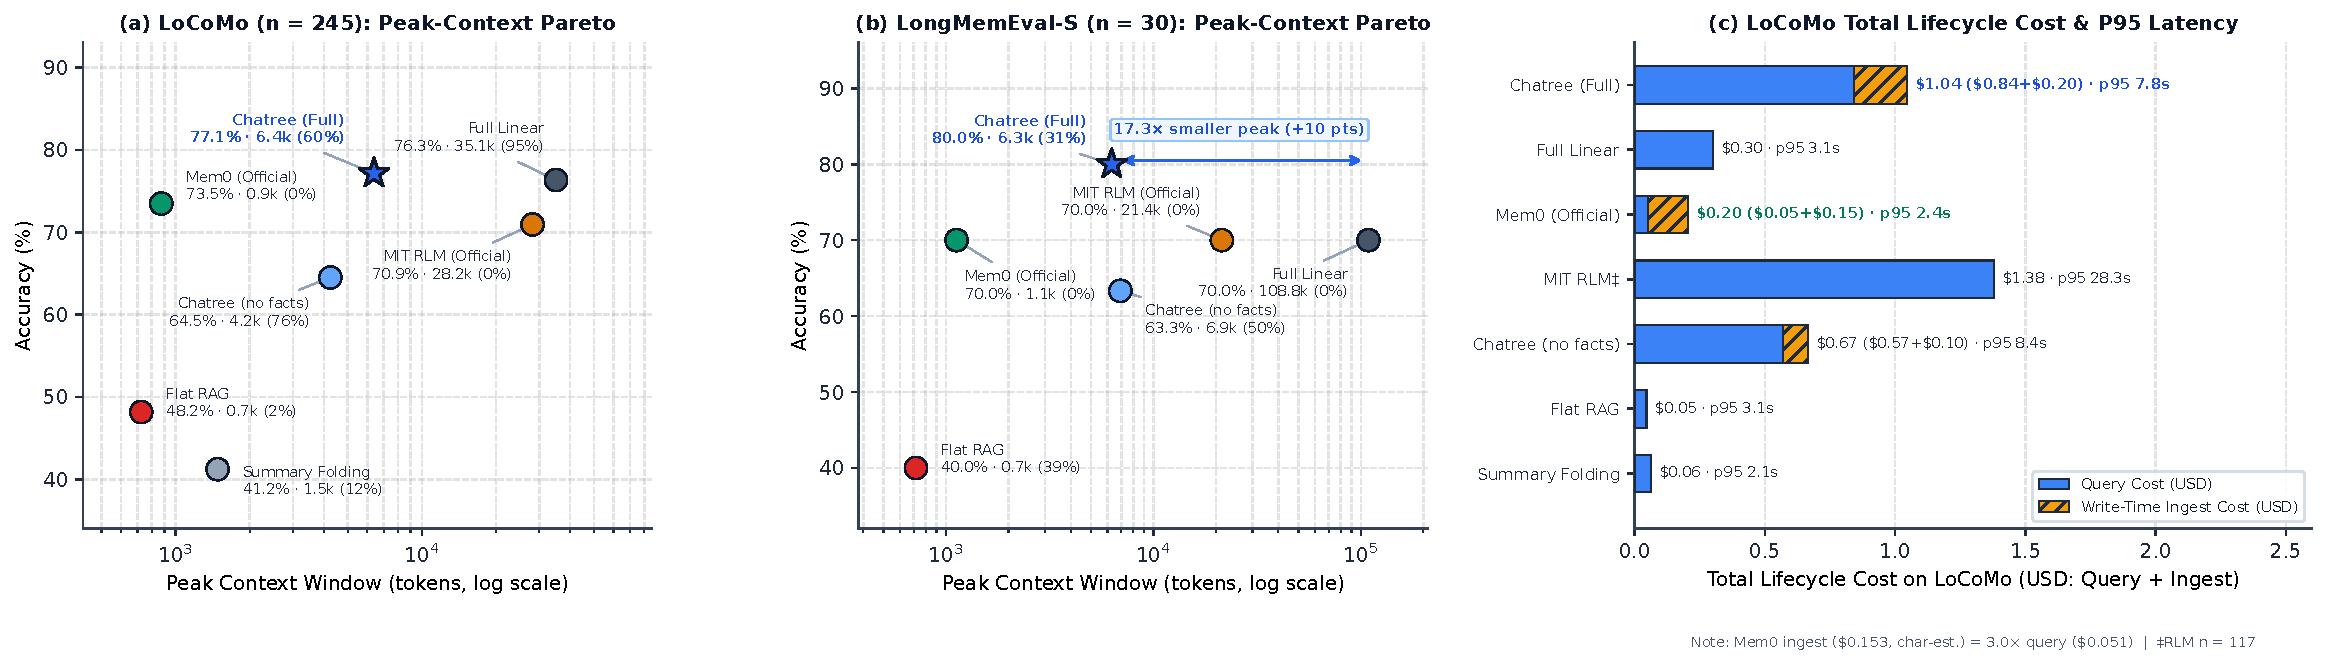
\includegraphics[width=\textwidth]{figures/fig3_pareto_efficiency.pdf}
  \caption{Accuracy vs.\ peak context on (a)~LoCoMo ($n=245$) and (b)~LongMemEval-S ($n=30$), and (c)~Total Lifecycle Cost (query + write-time ingest) with p95 latency on LoCoMo. Chatree sits on the upper-left Pareto frontier on both benchmarks.}
  \label{fig:pareto}
\end{figure*}

Chatree ranks first at \textbf{80.0\%} (+10~pts over Full Linear, Mem0, and RLM; +40~pts over Flat RAG, $p=0.0018^*$). Compared to Mem0 at 115k-token scale, Chatree gains \textbf{+40~pts on \texttt{knowledge-update}} (80\% vs.\ 40\%) and \textbf{+20~pts on \texttt{multi-session}} (60\% vs.\ 40\%), while costing \textbf{28\% less overall} (\$1.119 vs.\ \$1.555) and running 24\% faster on ingest (4,552s vs.\ 6,025s). Against Full Linear, Chatree cuts peak context by \textbf{17.3$\times$} (6,295 vs.\ 108,772 tokens) and cuts query cost by \textbf{3.8$\times$} (\$0.235 vs.\ \$0.882), while beating MIT RLM by \textbf{4.2$\times$ faster p95 latency} (7.69s vs.\ 31.98s).

\subsection{Why Architecture Matters vs.\ Mem0: Zero-Token Traces and Live Micro-Probes}
Standard Q\&A benchmarks mix together model luck, prompt wording, and real structural differences. To isolate what a branching tree can guarantee that a flat fact store cannot, Track~8 runs two clean tests (Table~\ref{tab:track8}):

\paragraph{Part A: Zero-Token Real-Framework Trace (\$0.00).}
We execute real Chatree alongside real unmodified \texttt{mem0ai==2.2.1} routed through a local OpenAI-compatible mock server (0 external API tokens):
\begin{itemize}
  \item \textbf{Prefix KV-cache stability (16 turns):} Given the exact same base system prompt and 16-turn dialogue, Chatree's tail-only context keeps an average \textbf{82.5\%} longest common token prefix across consecutive turns, compared to \textbf{0.7\%} when top-$k$ memories are injected at the start of the prompt—cutting effective billed input tokens by \textbf{69.4\%} under a standard 0.1$\times$ cached-read discount.
  \item \textbf{Measured write-time prompt overhead:} Inspecting installed \texttt{mem0ai==2.2.1} directly shows a \textbf{33,653-character} ($\sim$8,413-token) extraction system prompt sent on every \texttt{add()} call (plus a 5,310-character update prompt during reconciliation). Chatree runs 0 extra write calls during chat turns and caps cold-branch summarization at 7,500 characters—yielding 2.4$\times$--4.4$\times$ lower total USD at $N=200$ sessions.
  \item \textbf{Identical-lossiness probe traces:} Giving \emph{both} frameworks the exact same lossy distillation across three probes—(1)~recovering 4 incidental log/config literals omitted from summaries, (2)~propagating an upstream auth revision across $A \to B \to C$ when querying $C$ without mentioning ``auth'' or ``JWT,'' and (3)~silently archiving a MongoDB spike without typing a cancellation note—Chatree passes \textbf{8/8 (100\%)} while Mem0 passes \textbf{0/8 (0\%)}.
\end{itemize}

\paragraph{Part B: Live Head-to-Head Verification ($\sim$\$0.015).}
Running the exact same three probes live on \texttt{deepseek-chat} confirms the structural gap: Chatree scores \textbf{8/8 (100\%, 0 leaks, 78.7--81.9\% KV cache)} vs.\ unmodified \texttt{mem0ai==2.2.1} at \textbf{6/8 (75\%, 1 leak, 0.0\% KV cache)}.
\begin{itemize}
  \item On \textbf{Probe~3 (Silent Archiving)}, with no cancellation essay typed, unmodified Mem0 reported archived MongoDB prototype values (\texttt{rs\_ledger\_0}, \texttt{wiredTigerCacheSizeGB=24}) as active production configuration; Chatree returned 0\% leakage.
  \item On \textbf{Probe~2 (Transitive Staleness)}, Chatree automatically flagged both $B$ (1~hop) and $C$ (2~hops) stale when $A$ changed (2/2 vs.\ Mem0's 0/2), alerting $C$ immediately to block the release.
  \item On \textbf{Probe~1 (Tiny 12-Turn Verbatim Recall)}, both systems scored 4/4 live—honestly illustrating how Mem0 handles very short threads: its 33.6k-char prompt exploded 12 short turns into 13 verbose Qdrant memories (at 0\% KV cache). Once histories grow long enough to force real compression (as in Part~A and LongMemEval-S), dropped details cannot be recovered from a distilled store.
\end{itemize}

\begin{table}[t]
\centering
\caption{Track~8 zero-token structural trace (8A, \$0.00, real \texttt{mem0ai==2.2.1} local proxy) and live \texttt{deepseek-chat} verification (8B, $\sim$\$0.015).}
\label{tab:track8}
\scriptsize
\setlength{\tabcolsep}{2.6pt}
\resizebox{\linewidth}{!}{%
\begin{tabular}{@{}lcc@{}}
\toprule
\textbf{Diagnostic Check} & \textbf{Chatree} & \textbf{Mem0 (\texttt{2.2.1})} \\
\midrule
8A: 16-Turn Prefix Cacheability (LCP) & \textbf{82.5\%} {\tiny($-69\%$ tok)} & 0.7\% \\
8A: Measured Write-Prompt Size & \textbf{0/turn; 7.5k finish} & 33,653 chars/add \\
8A: Identical-Lossiness Probes 1--3 & \textbf{8/8 (100\%)} & 0/8 (0\%) \\
\midrule
8B Live: Probe 1 Verbatim Recall & \textbf{4/4} {\tiny(81.9\% cache)} & 4/4 {\tiny(0.0\% cache)} \\
8B Live: Probe 2 Transitive Stale ($A{\to}B{\to}C$) & \textbf{2/2} {\tiny(2/2 flags)} & 1/2 {\tiny(0/2 flags)} \\
8B Live: Probe 3 Silent Archive Quarantine & \textbf{2/2} {\tiny(0 leaks)} & 1/2 {\tiny(\textbf{1 leak})} \\
\textbf{8B Live Combined Rollup} & \textbf{8/8 (100\%)} & 6/8 (75\%) \\
\bottomrule
\end{tabular}%
}
\end{table}

\subsection{Non-Destructive Compaction and Live Multi-Turn Use}
Figure~\ref{fig:compaction} summarizes Tracks~6 and~5.

\begin{figure*}[t]
  \centering
  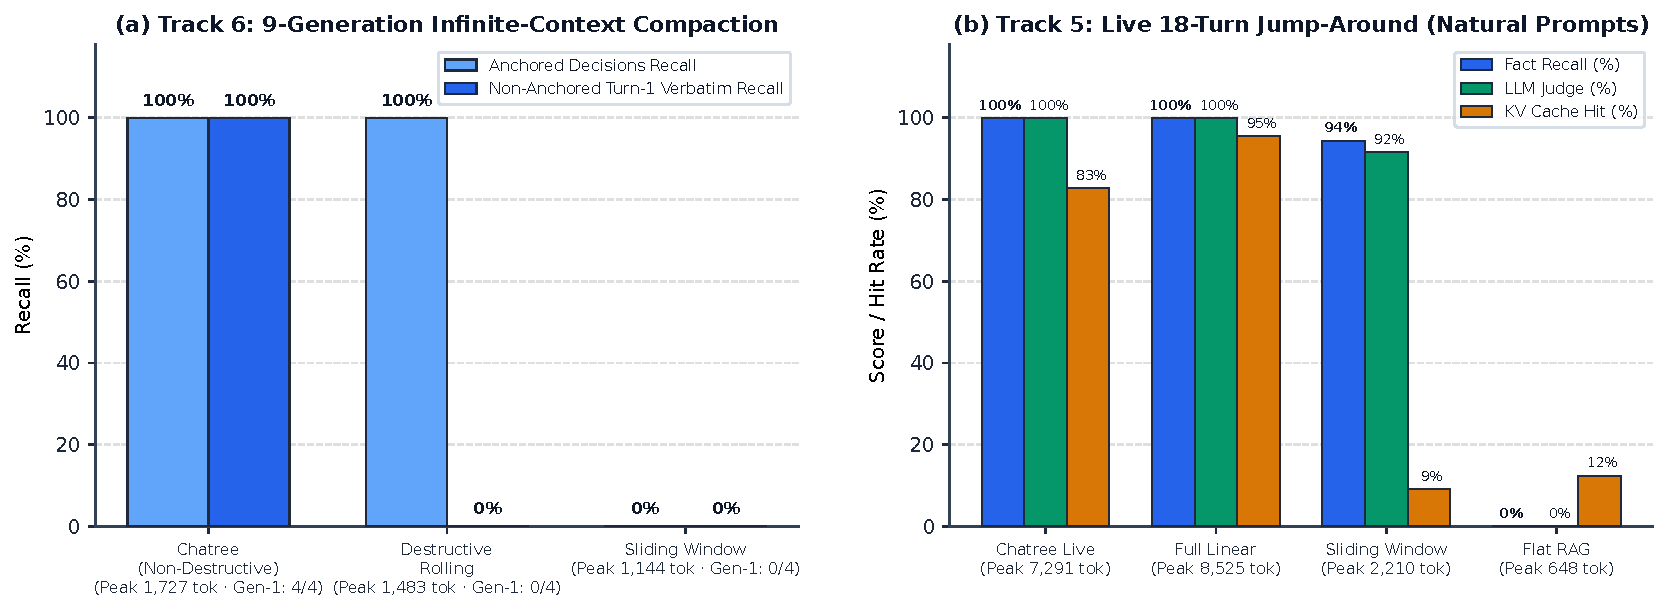
\includegraphics[width=\textwidth]{figures/fig5_compaction_and_live.pdf}
  \caption{(a)~9-generation compaction benchmark: Chatree keeps 100\% recall on both anchored decisions and un-anchored Turn-1 details at 1,727 peak tokens, whereas rolling compaction drops to 0\% on un-anchored details. (b)~18-turn live multi-topic chat under natural prompts.}
  \label{fig:compaction}
\end{figure*}

\paragraph{9-Generation Compaction (Track~6).}
Across 9 consecutive compactions (Table~\ref{tab:compaction}), Chatree holds working context steady at \textbf{1,723 tokens} while achieving \textbf{100\% recall} on both anchored security decisions and un-anchored Turn-1 diagnostic constants (by querying the untouched Turn-1 ancestor). Destructive rolling compaction keeps anchored decisions (100\%) but loses every un-anchored Turn-1 detail (\textbf{0\%}), and a sliding window loses both (\textbf{0\%}).

\begin{table}[t]
\centering
\caption{9-generation live compaction benchmark (\texttt{deepseek-chat}).}
\label{tab:compaction}
\scriptsize
\setlength{\tabcolsep}{3.0pt}
\resizebox{\linewidth}{!}{%
\begin{tabular}{@{}lccccrr@{}}
\toprule
\textbf{System} & \textbf{Comp.} & \textbf{Anch.} & \textbf{Un-Anch.} & \textbf{All} & \textbf{Peak} & \textbf{Gen-1} \\
\midrule
\textbf{Chatree (Non-Destr.)} & 9 & \textbf{100\%} & \textbf{100\%} & \textbf{100\%} & 1,727 & \textbf{4/4} \\
Destructive Rolling & 6 & \textbf{100\%} & 0\% & 50\% & 1,483 & 0/4 \\
Sliding Window & 0 & 0\% & 0\% & 0\% & 1,144 & 0/4 \\
\bottomrule
\end{tabular}%
}
\end{table}

\paragraph{Live 18-Turn Jump-Around Chat (Track~5).}
Using natural user prompts with zero mention of trees or tools, live Chatree autonomously spawns 4 branches, makes 5 jumps and 11 read-only lookups, and achieves \textbf{100\% recall}, \textbf{1.00 judge score}, \textbf{0\% dead-end leakage}, \textbf{82.7\% KV-cache hits}, and lower peak context than linear chat (7,291 vs.\ 8,525 tokens). Sliding window drops to 94.4\% recall (9.1\% cache) and flat RAG fails (0\%). Importantly, on this short 18-turn thread, Chatree spends more total input tokens than linear chat (360k vs.\ 76.5k; \$0.034 vs.\ \$0.006), illustrating that tree orchestration pays off beyond a branching/length crossover rather than in brief linear chats.

\subsection{Controlled Stress Tests, Ablations, and Token Crossover}

\paragraph{Non-Monotonic Engineering Workspaces (Track~7, $n=36$).}
Across 6 multi-sprint projects (80 sessions including 18 scrapped prototypes with explicit textual cancellation messages; Table~\ref{tab:track7}), Chatree scores \textbf{100\% (36/36)} at 68.6\% KV-cache hits—significantly outperforming MIT RLM (77.8\%, $p=0.0078^*$) and Flat RAG (36.1\%, $p<10^{-4}$), and beating Summary Folding (88.9\%). At this small 3.7k-token scale with explicit cancellations, Full Linear and Mem0 also score 100\%, confirming that their failures surface either when dead ends are archived silently (Track~8) or when histories scale to 35k--115k tokens (LoCoMo and LongMemEval-S).

\begin{table}[t]
\centering
\caption{Track~7 engineering spec-reversal benchmark ($n=36$, 80 sessions across 6 projects). $^*$ denotes $p < 0.05$ vs.\ Chatree.}
\label{tab:track7}
\scriptsize
\setlength{\tabcolsep}{2.6pt}
\resizebox{\linewidth}{!}{%
\begin{tabular}{@{}lccccrr@{}}
\toprule
\textbf{System} & \textbf{All} & \textbf{Rev.} & \textbf{Verb.} & \textbf{Synth.} & \textbf{Total USD} & \textbf{$p$} \\
\midrule
\textbf{Chatree} & \textbf{100\%} & \textbf{100\%} & \textbf{100\%} & \textbf{100\%} & \$0.099 & ref \\
Full Linear & \textbf{100\%} & \textbf{100\%} & \textbf{100\%} & \textbf{100\%} & \$0.011 & 1.000 \\
Mem0 (\texttt{2.2.1}) & \textbf{100\%} & \textbf{100\%} & \textbf{100\%} & \textbf{100\%} & \$0.030 & 1.000 \\
Summary Folding & 88.9\% & 100\% & 75.0\% & 83.3\% & \$0.020 & .125 \\
MIT RLM (\texttt{0.1.3}) & 77.8\% & 66.7\% & 75.0\% & 66.7\% & \$0.111 & \textbf{.0078$^*$} \\
Flat Hybrid RAG & 36.1\% & 33.3\% & 25.0\% & 0.0\% & \textbf{\$0.008} & \textbf{$<$.0001$^*$} \\
\bottomrule
\end{tabular}%
}
\end{table}

\paragraph{5-Family Stress Suite, Ablations, and $K$-Scaling Crossover (Tracks~1 \&~2).}
On Track~1 (Table~\ref{tab:track1}), Chatree passes \textbf{8/8 (100\%)} with 0\% leakage and 0\% stale contradictions, whereas Flat RAG, Summary Folding, and Chatree-without-staleness all fail the multi-hop revision test. Figure~\ref{fig:crossover} shows Track~2's scaling curve and ablations:
\begin{itemize}
  \item \textbf{Total-token crossover at $K=8$:} Across $K \in \{2,4,8\}$ distractor branches, Chatree holds 100\% pass and nearly flat peak context ($707 \to 767 \to 957$ tokens). At $K=8$, Chatree crosses below Full Linear in \emph{cumulative} input tokens (\textbf{29.6k vs.\ 39.7k}) and median latency (\textbf{1.19s vs.\ 1.42s}), while Sliding Window drops to 0\%.
  \item \textbf{Ablations:} Disabling read-only branch lookups collapses strict pass rate to \textbf{0.0\%} ($p=0.0312^*$). Disabling staleness tracking or materiality gating introduces 14.3\% stale errors, and disabling multi-hop transitivity drops accuracy to 71.4\%.
\end{itemize}

\begin{table}[t]
\centering
\caption{Track~1 5-family stress suite strict pass rates and peak root tokens (\texttt{deepseek-chat}).}
\label{tab:track1}
\scriptsize
\setlength{\tabcolsep}{3.0pt}
\resizebox{\linewidth}{!}{%
\begin{tabular}{@{}lcccc@{}}
\toprule
\textbf{Scenario Family} & \textbf{Linear} & \textbf{Flat RAG} & \textbf{Folding} & \textbf{Chatree} \\
\midrule
Distractor Scaling ($K=4$) & 2/2 {\tiny(2.5k)} & 0/2 {\tiny(0.8k)} & 0/2 {\tiny(0.9k)} & \textbf{2/2} {\tiny(0.9k)} \\
Proposal vs.\ Decision     & 2/2 {\tiny(2.3k)} & 1/2 {\tiny(0.9k)} & 0/2 {\tiny(0.9k)} & \textbf{2/2} {\tiny(1.2k)} \\
Multihop Revision ($A{\to}B{\to}C$) & 1/1 {\tiny(3.0k)} & 0/1 {\tiny(1.1k)} & 0/1 {\tiny(1.1k)} & \textbf{1/1} {\tiny(1.1k)} \\
Unscripted Agentic Policy  & 1/1 {\tiny(1.6k)} & --- & --- & \textbf{1/1} {\tiny(4.2k)} \\
Crossover ($B=4, T=3$)     & 2/2 {\tiny(6.6k)} & 2/2 {\tiny(1.2k)} & 0/2 {\tiny(1.2k)} & \textbf{2/2} {\tiny(1.2k)} \\
\midrule
\textbf{Total Strict Pass} & \textbf{8/8 (100\%)} & 3/7 (43\%) & 0/7 (0\%) & \textbf{8/8 (100\%)} \\
\bottomrule
\end{tabular}%
}
\end{table}

\begin{figure*}[t]
  \centering
  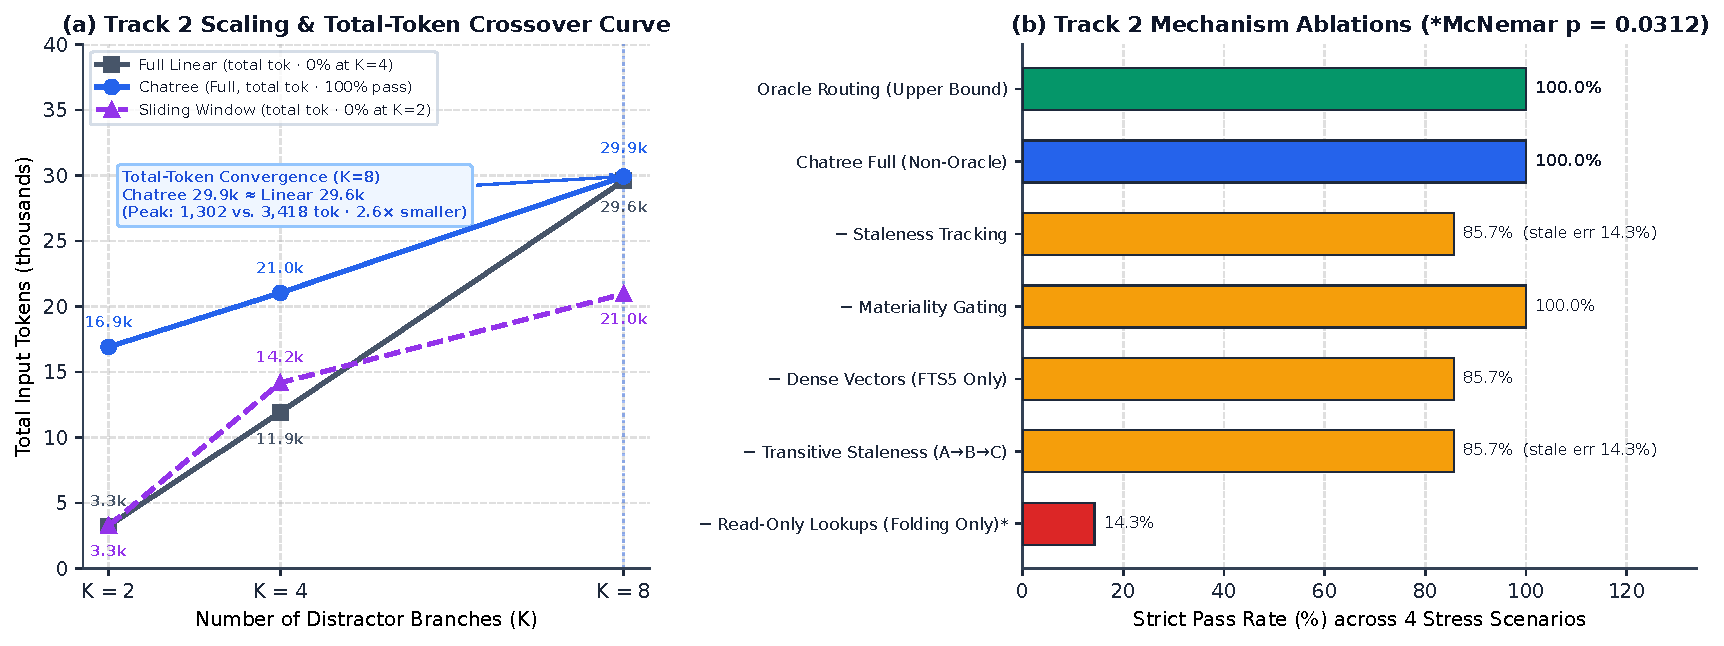
\includegraphics[width=\textwidth]{figures/fig4_crossover_and_ablations.pdf}
  \caption{Track~2 scaling and ablations: (a)~Chatree crosses below linear chat on total input tokens at $K=8$ distractor branches while sustaining 100\% accuracy; (b)~single-feature ablations confirm read-only branch lookups are essential ($p=0.0312^*$).}
  \label{fig:crossover}
\end{figure*}

% ============================================================================
% 6. LIMITATIONS & WHEN TO USE CHATREE
% ============================================================================
\section{Limitations and Practical Trade-Offs}

Chatree is not free and not the right tool for every chat:
\begin{enumerate}
  \item \textbf{Short linear threads:} Under roughly 10k tokens and a single topic, plain linear chat is faster and cheaper (as seen on our 18-turn jump-around benchmark). Tree orchestration pays off once conversations branch heavily, exceed context limits, or accumulate dozens of sessions.
  \item \textbf{Single-model evaluation and sample sizes:} All live runs use \texttt{deepseek-chat} on a single seed, including LLM judging on Tracks~1--7 (Track~8A is zero-token deterministic and Track~8B uses verifiable token/leakage checks). Our LongMemEval-S evaluation is a 30-item stratified subset, and MIT RLM completed 117/245 LoCoMo questions before an API pause (paired McNemar tests use the exact intersection). Cross-family judging and full-split runs remain future work.
  \item \textbf{Interactive vs.\ structured querying:} External benchmarks call Chatree's structured multi-hop query engine directly, whereas live interactive chats rely on the LLM deciding when to branch or look up siblings.
  \item \textbf{Context overflow beyond 128k tokens:} LongMemEval-S ($\sim$115k tokens) still fits inside DeepSeek's 128k window; testing the 1.5M-token LongMemEval-M split is supported by our runner and left for future work.
  \item \textbf{Hosted cache TTL and SQLite scale:} Hosted prompt caches expire after $\sim$5--10 minutes, so prefix stability saves money mainly during active sessions or on self-hosted engines. Single-process SQLite fits local workspaces well, while large multi-tenant deployments will need an ANN/Postgres backend.
\end{enumerate}

% ============================================================================
% 7. CONCLUSION
% ============================================================================
\section{Conclusion}

Managing long LLM conversations does not require choosing between a bloated linear transcript and a lossy bag of extracted facts. Organizing history as a tree of isolated branches—with cheap summaries and dated facts for search, read-only lookups over verbatim history for exact details, dependency tracking for upstream changes, silent archiving for dead ends, and tail-only metadata for prefix caching—gives models bounded working context without throwing away provenance. Across LoCoMo, LongMemEval-S, multi-generation compaction, and direct comparisons against Mem0 and MIT RLM, this simple structure improves accuracy on long, evolving workflows while keeping context size and total lifecycle cost under control.

\paragraph{Code and Artifacts.}
All code, 111 zero-key tests, raw evaluation checkpoints, zero-token simulation scripts, and figure generators are open-source at \texttt{https://github.com/shervinemp/Chatree}.

\bibliographystyle{plainnat}
\bibliography{references}

\end{document}
